\documentclass[conference]{IEEEtran}
\IEEEoverridecommandlockouts
% The preceding line is only needed to identify funding in the first footnote.  If that is unneeded, please comment it out.
\usepackage{cite}
\usepackage{amsmath,amssymb,amsfonts}
\usepackage{algorithmic}
\usepackage{graphicx}
\usepackage{textcomp}
\usepackage{xcolor}
\def\BibTeX{{\rm B\kern-.05em{\sc i\kern-.025em b}\kern-.08em
    T\kern-.1667em\lower.7ex\hbox{E}\kern-.125emX}}

\usepackage{makeidx}
\usepackage{times}
\usepackage{epsf}
\usepackage{epsfig}
\usepackage{graphics}
\usepackage{color}
\usepackage{url}

\usepackage{balance}  % for  \balance command ON LAST PAGE  (only there!)

%\usepackage[english]{babel} % otherwise, \cite doesn't work with sig-alternate/acm_proc_article-sp
\usepackage{txfonts}
%\usepackage{multiFloats}

\usepackage{pslatex}
\usepackage[all]{xy}

% wrap text around (floating) figures
\usepackage{wrapfig}
%\setlength{\wrapoverhang}{0mm}

% For the nicer display of verbatim text
\usepackage{colortbl} % \definecolor
\usepackage{fancyvrb}
\definecolor{grayborder}{rgb}{0.75,0.75,0.75}
\DefineVerbatimEnvironment
{verb}{Verbatim}
{fontsize=\scriptsize,tabsize=4,frame=single,framesep=1mm,rulecolor=\color{grayborder},baselinestretch=1,commandchars=\\\{\}}
\DefineVerbatimEnvironment
{verb2}{Verbatim}
{fontsize=\scriptsize,tabsize=4,frame=single,framesep=1mm,rulecolor=\color{grayborder},baselinestretch=1,commandchars=\\<>}
\DefineVerbatimEnvironment
{verbnocommand}{Verbatim}
{fontsize=\scriptsize,tabsize=4,frame=single,framesep=1mm,rulecolor=\color{grayborder},baselinestretch=1}

\def\Skip{\par\medskip\nobreak\noindent}

\begin{document}

\title{Database Resource Allocation Based on Resilient Intermediates}

\author{
\IEEEauthorblockN{Martin Kersten, Ying Zhang, Pavlos Katsogridakis, \\Panagiotis Koutsourakis and Joeri van Ruth}
\IEEEauthorblockA{
\textit{MonetDB Solutions}\\
Amsterdam, The Netherlands \\
\textit{\textless lastname\textgreater}@monetdbsolutions.com}
}

\maketitle

\begin{abstract} 
%What is the market pitch? 
Scale-out of big data analytics applications often does not pay off due to the poor performance in response time  and the increasing bill due to a longer execution time on a resource limited machine.
To enable a stable DBMS workload environment it helps to maintain several virtual machines with difference resource configurations (CPU, memory, disk, etc) hosting part of the database, so that users can send their tasks to those machines that have the best price/performance characteristics.
This, however, requires a method to decide which VM should be used for a given query.

When choosing the VM, the memory usage of a query is a particularly important factor, especially for the main-memory (optimised) DBMSs which are generally used for analytical queries today.
In this paper, we introduce MALCOM, a memory footprint predictor for queries based on resilient intermediates in MonetDB.
Unlike traditional cost-based approaches, MALCOM uses an empirical approach (i.e. using the memory usage information of queries executed in the past) to incrementally update its model to improve its predictions.
Our preliminary experiment results show that this approach is robust against varying data distributions.
\end{abstract} 

\section{Introduction}
\label{Introduction} 
Since the start of database research, database designers have keenly looked at the opportunities to use large, distributed processing platforms. Cluster-based products are readily available, such as in appliance products from Oracle Exadata, SQL Parallel Data Warehouse, IBM Blu and Teradata, but they are often limited to a few tens of compute nodes.
A plethora of research activities has shown that in all but the simplest cases achieving a good performance is at least hard, especially when a query involves joins spread over multiple compute nodes and thus requires expensive data exchange.

The predominant way out nowadays, taken by NoSQL systems such as Casandra and Impala, is to address part of the problem space by focusing on select-aggregate queries.
This choice has proven to be pivotal to support big data analytics in many real-world circumstances, as shown by the widespread use of Apache Spark.
The basic abstraction in Spark is a Resilient Distributed Dataset (RDD), which represents an immutable and partitioned collection of elements that can be operated on in parallel using operators, such as map, filter, persist and aggregates.
%Moreover, an RDD is the basic component to be exchanged between operators, threads, cores and machines.
%In essence, an RDD can be seen as a relational table used for interoperability, an approach that can be traced back to Microsoft's ODE, which has been used for decades to exchange data between DBMS and its applications.
%Similar functional abstractions can nowadays be found in R's Data Frames and Python Pandas.

Although in many cases it is easy to scale-up for improved response time, partitioning a database to benefit from a low cloud service price tag and to overcome resource limitations of smaller machines is still a much sought-after skill.
This product space is addressed by Snowflake and AWS Redshift.
Snowflake has been designed from a cloud perspective, taking resource management as its key driving factor.
It conceptually provides every user with a complete copy of the database and relies on multi-level caching.
AWS Redshift is an improved version of PostgreSQL, which has been further tuned towards better I/O bandwidth use.

In this paper we take a fresh look at resource allocation for query processing in the context where intermediates in a query plan are fully materialised before passed on towards the next operator.
This model fits not only the Apache Spark programming model, but also the query execution model of our database system MonetDB\footnote{\url{www.monetdb.org}}.
Resilient intermediates provide new avenues for query optimisation and scheduling as its underlying computation model is based on materialisation of all intermediate steps.
Furthermore, in most practical business analytic cases the past is a reasonable predictor of the future.

The main contributions of this paper are
\begin{itemize}
	\item we develop a simulator, called {\sc malcom} to predict the memory footprint for queries based on resilient intermediates in MonetDB.
	\item We demonstrate that the approach is robust against varying data distributions.
	\item We demonstrate the opportunities using an extensive evaluation against TPC-H and a real-world data set.
\end{itemize}

The approach taken here differs from traditional cost-based query optimisers deployed in distributed database systems by learning about actual resource claims over time, i.e. after each query execution we have precise knowledge of the resources used.
This information can be harvested and used to predict future operations of a similar nature.
The rationale stems from the common knowledge that any database application environment has a limited number of ``business transactions'' or ``business intelligence templates'' where only some parameters are changed with each call.
%This knowledge has been used in the past to drive development of DBA wizards~\cite{ms_wizards} for index selection by humans and self-tuning optimisers~\cite{IBM} to avoid expensive join paths in individual queries.

\Skip
\textbf{Paper Outline.}
Section~\ref{sec:background} provides a short overview of the MonetDB architecture. % and the projects involved.
Section~\ref{sec:malcolm} introduces the components and algorithms for our resource estimator {\sc malcom}.
Section~\ref{sec:evaluation} illustrates the effectiveness of our approach in two use cases: TPC-H and air traffic.

\section{Background}
\label{sec:background} 
In this section we introduce the query execution engine of MonetDB and the performance information available for our task.

\subsection{MonetDB Architecture}
%Recap some MonetDB stuff on how queries are compiled.
MonetDB is a widely used columnar DBMS that internally uses resilient intermediates to break up query processing in well identifying steps. 
A query plan is broken up into independent steps, glued together into a dataflow dependency graph.
The dataflow graph is greedily consumed by the database kernel assigning a dedicated core to each operation.
The resource pressure is kept at a minimum by trimming down the degree of parallel processing when the main memory resource is heavily used.
% The system can be instructed to produce an event record for each completed instruction.
% This provides a.o. insights into the input/output sizes and timing.

\begin{figure}[t]
    \centering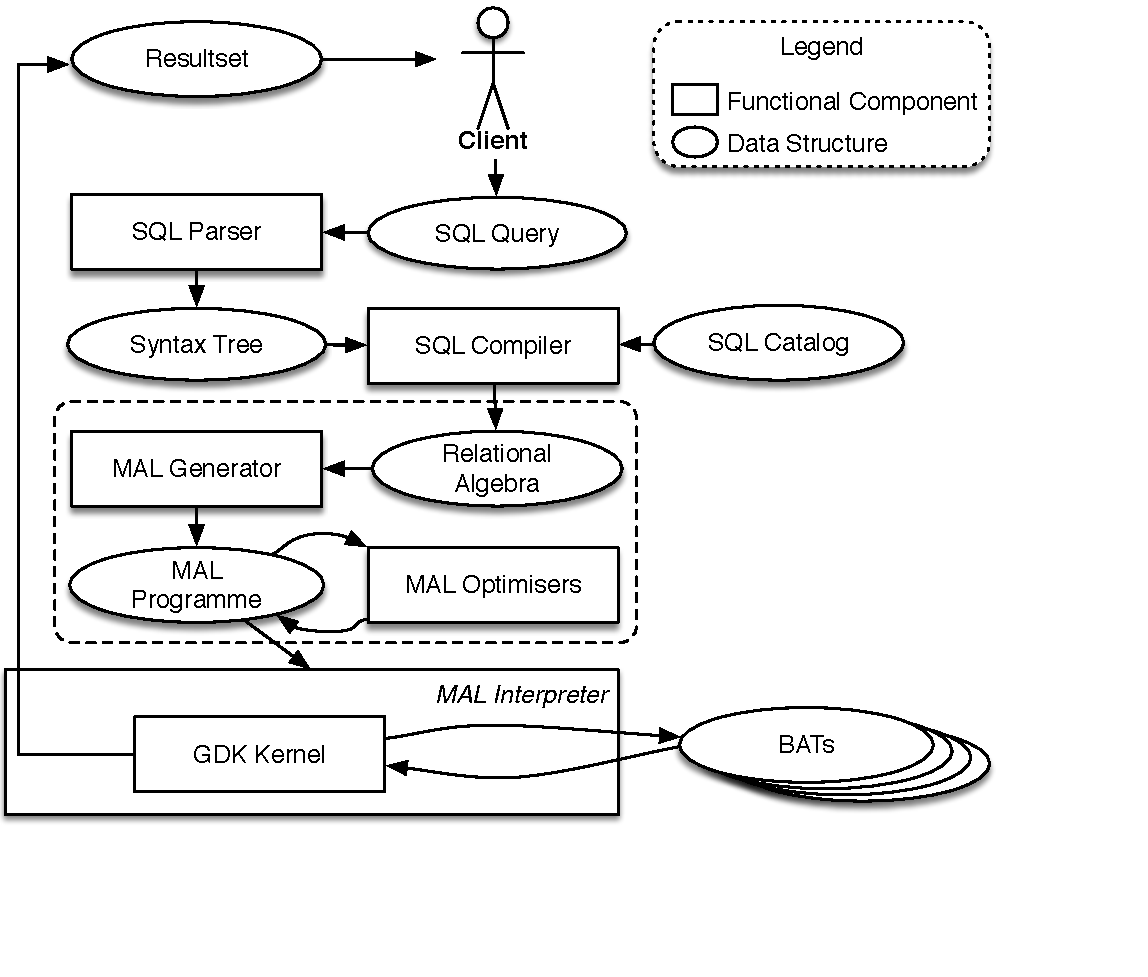
\includegraphics[width=\columnwidth]{Figures/MDB_impl_arch.pdf}
    \caption{MonetDB query execution architecture.}
    \label{fig:mdb_arch}
\end{figure}

%\subsection{Architecture}
Figure~\ref{fig:mdb_arch} illustrates the components of MonetDB to execute an SQL query.
{\sc mal} (MonetDB Assembly Language) is the MonetDB internal language into which SQL queries are compiled and executed.
The SQL Parser and {\sc mal} Optimiser deploy well-known rewriting rules (e.g. parallelisation, and dead code/common expression/constant elimination) to reduce the intermediate sizes and processing time.
They do not rely on any cost-model or pre-computed statistics.

The middle layer (in the dashed box) is a sequence of specialised optimisers that morph a logical plan produced by the SQL compiler into a physical execution plan containing relational operators expressed in {\sc mal} statements.
The bottom layer (under the dashed box) contains the implementation of the {\sc mal} statements.
Each operator takes as input the resilient intermediates produced by operators executed before or the persistent data on disk.
%The actual implementation is often quite complex, because each operator can be implemented in a multitude of ways.
%Since the operator has full knowledge on the actual parameters, it becomes easy to select the proper path.
%Some operators even perform a sampling step before making a choice on the preferred algorithm.

As an example, consider this simple SQL query: \texttt{\small SELECT COUNT(*) FROM sys.\_tables}, which is eventually translated into a physical execution plan in {\sc mal} statements to be executed by the MonetDB kernel.
The box below show an excerpt of the plan:
\begin{verb}
C_5=<tmp_1524>[92]:bat[:oid] := sql.tid("sys":str, "_tables":str);
X_8=<tmp_147>[99]:bat[:int] := \textbf{sql.bind}
     (\textbf{"sys"}:str, \textbf{"_tables"}:str, \textbf{"id"}:str);
X_17=<tmp_1477>[92]:bat[:int] := \textbf{algebra.projection}
     (C_5=<tmp_1524>[92]:bat[:oid], X_8=<tmp_147>[99]:bat[:int]);
X_18=92:lng := \textbf{aggr.count}(X_17=<tmp_1477>[92]:bat[:int]);
sql.resultSet("sys.L3":str, "L3":str, "bigint":str, 
              64:int, 0:int, 7:int, X_18=92:lng);
\end{verb}

The {\sc mal} language is purely designed as intermediate language to express the operations.
Generally, a {\sc mal} statement is an assignment of the form:
\begin{verb}
VAR=<FILENAME>[COUNT]:VAR_TYPE := 
     MOD.FUNC(PARAM1 = <FILENAME>[COUNT]:PARAM1_TYPE, ...);
\end{verb}

Every function belongs to a module.
The arguments are either typed scalar values (\texttt{\small :type}) or a reference to a column (\texttt{\small :bat[:type]}).
If a variable (\texttt{\small VAR}) refers to a column, which can be memory mapped, it is also tagged with its base \texttt{\small FILENAME} on disk and the number of values in this column (\texttt{\small COUNT}).

The above {\sc mal} program is straightforward.
It first loads (\texttt{\small sql.bind}) and projects (\texttt{\small algebra.projection}) the data of one column (\texttt{\small sys.\_tables.id}) from the disk.
Then the data is passed to \texttt{\small aggr.count} to compute the \texttt{\small COUNT}.
Finally, \texttt{\small sql.resultSet} emits the query result.
The {\sc mal} statements play an important role in {\sc malcolm}: before a query execution, one can pass the query's execution plan in MAL to {\sc malcolm} to get an estimation of the memory footprint of this query; and after a query execution, one can pass the query's execution trace to {\sc malcolm}.
The trace is also expressed as {\sc mal} statements, but they now contain various information of the actual query execution, such as the execution time of each {\sc mal} statement and the number of values contained in each input and output paramter. 
Given such a trace, {\sc malcolm} can subsequently collect execution statistics per {\sc mal} statement and update its model.

%\begin{table}
\begin{figure}[t]
\renewcommand{\arraystretch}{1.1}
\renewcommand{\tabcolsep}{3pt}
\centering
{\scriptsize
\begin{tabular}{|l@{~}l|}
\hline
\textbf{JSON object at ``start'' time}    &   \textbf{JSON object at ``done'' time}                                      \\
\hline                                                                                                                                 
\renewcommand{\arraystretch}{0.9}\renewcommand{\tabcolsep}{3pt}\{``source'':``trace'', &   \{``source'':``trace'',       \\
% ~{\color{red}``clk'':1767476753919,}                     &   ~ {\color{red}``clk'':1767476754150,}                      \\
 ~{\color{red}``ctime'':1528314717302449,}                &   ~ {\color{red}``ctime'':1528314717302680,}                 \\
% ~``thread'':8,                                           &   ~ ``thread'':8,                                            \\
% ~``function'':``user.s4\_2'',                            &   ~ ``function'':``user.s4\_2'',                             \\
% ~``pc'':9,                                               &   ~ ``pc'':9,                                                \\
% ~``tag'':248,                                            &   ~ ``tag'':248,                                             \\
 ~``module'':``algebra'',                                 &   ~ ``module'':``algebra'',                                  \\
 ~``instruction'':``projection'',                         &   ~ ``instruction'':``projection'',                          \\
% ~``session'':``b4a92225-127d-4a1f-b2ef-...'',            &   ~ ``session'':``b4a92225-127d-4a1f-b2ef-...'',             \\
 ~{\color{red}``state'':``start'',}                       &   ~ {\color{red}``state'':``done'',}                         \\
 ~{\color{red}``usec'':0,}                                &   ~ {\color{red}``usec'':230,}                               \\
 ~``rss'':87,                                             &   ~ ``rss'':87,                                              \\
 ~``size'':0,                                             &   ~ ``size'':0,                                              \\
 ~{\color{red}``nvcsw'':1,}                               &   ~                                                          \\
 ~``stmt'':"X\_17?:= \textbf{algebra.projection}(?);'',   &   ~ ``stmt'':"X\_17?:= \textbf{algebra.projection}(?);'',    \\
% ~``short'':"X\_17[0]:= projection(?, ?)'',               &   ~ ``short'':"X\_17[0]:= projection(?, ?)'',                \\
% ~``prereq'':[4,8],                                       &   ~ ``prereq'':[4,8],                                        \\
 ~\textbf{``ret"}:[\{                                     &   ~ ``ret'':[\{                                              \\
 ~   ``index'':``0'',                                     &   ~    ``index'':``0'',                                      \\
 ~   ``name'':"X\_17'',                                   &   ~    ``name'':"X\_17'',                                    \\
 ~   ``alias'':``sys.\_tables.id'',                       &   ~    ``alias'':``sys.\_tables.id'',                        \\
 ~   ``type'':``bat[:int]'',                              &   ~    ``type'':``bat[:int]'',                               \\
 ~                                                        &   ~ {\color{red}``kind'':``transient'',}                     \\
% ~   {\color{red}``bid'':``0'',}                          &   ~    {\color{red}``bid'':``837'',}                         \\
 ~   {\color{red}``count'':``0'',}                        &   ~    {\color{red}``count'':``92'',}                        \\
 ~   {\color{red}``size'':0,}                             &   ~    \textbf{\color{red}``size'':368,}                     \\
 ~   \textbf{``eol'':0}\}],                               &   ~    \textbf{``eol'':0}\}],                                \\
 ~\textbf{``arg"}:[\{                                     &   ~ \textbf{``arg"}:[\{                                      \\
 ~~~~   ``index'':``1'',                                  &   ~~~~    ``index'':``1'',                                   \\
 ~~~~   ``name'':"C\_5'',                                 &   ~~~~    ``name'':"C\_5'',                                  \\
% ~~~~   ``type'':``bat[:oid]'',                           &   ~~~~    ``type'':``bat[:oid]'',                            \\
 ~~~~   ``kind'':``transient'',                           &   ~~~~    ``kind'':``transient'',                            \\
 ~~~~   ``bid'':``863'',                                  &   ~~~~    ``bid'':``863'',                                   \\
 ~~~~   ``count'':``92'',                                 &   ~~~~    ``count'':``92'',                                  \\
 ~~~~   ``size'':736,                                     &   ~~~~    ``size'':736,                                      \\
 ~~~~   \textbf{``eol'':1}\},                             &   ~~~~    \textbf{``eol'':1}\},                              \\
 ~~  \{``index'':``2'',                                   &   ~~   \{``index'':``2'',                                    \\
 ~~~~   ``name'':"X\_8'',                                 &   ~~~~    ``name'':"X\_8'',                                  \\
% ~~~~   ``alias'':``sys.\_tables.id'',                    &   ~~~~    ``alias'':``sys.\_tables.id'',                     \\
% ~~~~   ``type'':``bat[:int]'',                           &   ~~~~    ``type'':``bat[:int]'',                            \\
% ~~~~   ``kind'':``persistent'',                          &   ~~~~    ``kind'':``persistent'',                           \\
% ~~~~   ``bid'':``103'',                                  &   ~~~~    ``bid'':``103'',                                   \\
% ~~~~   ``count'':``99'',                                 &   ~~~~    ``count'':``99'',                                  \\
% ~~~~   ``size'':396,                                     &   ~~~~    ``size'':396,                                      \\
 ~~~~   ...                                               &   ...                                                        \\
 ~~~~   \textbf{``eol'':1}\}]\}                           &   ~~~~    \textbf{``eol'':1}\}]\}                            \\
\hline
\end{tabular}
}
\caption{JSON profiling objects produced for an \texttt{\small algebra.projection} operation.}
\label{fig:json_obj}
%\end{table}
\end{figure}

\subsection{MonetDB Profiling Information}

The MonetDB kernel can be instructed to emit profiling events for the execution of {\sc mal} statements, e.g. by establishing a connection using MonetDB's profiling tool.
% Every {\sc mal} function comes with two event records: one taken at the beginning and another upon completion of the operation.
%The event record contains details on the arguments passed, their type and size.
%%Wherever possible the arguments are linked with the underlying persistent column.
%Intermediate columns are nameless and we can only rely on their types and cardinalities.
%Upon completion, we also know the exact size of the result and the elapsed time.
%It can render the profiling events in two different formats: either as a  plain text tuple (one tuple per event) or as JSON objects (one object per event).
Figure~\ref{fig:json_obj} shows the before/after profiling events produced for the \texttt{\small algebra.projection} operation when executing the {\sc mal} program above.
The left column shows the event at the \texttt{\small "start"} and the right column the event when the operation is \texttt{\small "done"}.
Differences between the two objects are marked in red.
Of most interest to our estimation are the properties shown for the arguments (\texttt{\small "arg"}) and return variables (\texttt{\small "ret"}).
For instance, in a \texttt{\small "ret"} object, the field \texttt{\small "size"} is a good estimation of how much memory the result set of this function consumes; while in an \texttt{\small "arg"} object, the field \texttt{\small "eol":1} indicates this argument has reached its end-of-life.
This information together with the \texttt{\small "size"} allows us to estimate how much memory is freed after this operation.

%In principle we should collect all possible events as a basis for building an optimizer/simulator.
%Although the MonetDB kernel knows $>$10K operator/type specific signatures, the SQL front-end only needs a few tens of operator templates.
%For the TPC-H benchmark ca. 60 {\sc mal} operations are sufficient.

%\begin{figure}
%\begin{verb} 
%21.83 %       1332 calls algebra.projection
%12.91 %        768 calls mat.packIncrement
% 9.60 %        712 calls algebra.projectionpath
% 7.58 %        558 calls sql.bind
% 7.45 %        519 calls batcalc.*
% 7.25 %        435 calls algebra.join
% 5.48 %        330 calls bat.append
% 4.52 %        420 calls algebra.thetaselect
% 3.44 %        234 calls sql.bind_idxbat
% 3.34 %        223 calls algebra.select
% 2.49 %        179 calls sql.tid
% 2.46 %        144 calls batcalc.!=
% 2.06 %        138 calls aggr.subsum
% 1.98 %        218 calls bat.mergecand
% 1.30 %         74 calls sql.projectdelta
% 1.06 %         74 calls group.groupdone
% 1.06 %         75 calls bat.new
% 0.92 %         53 calls batcalc.==
% 0.90 %         72 calls batcalc.-
% 0.78 %         39 calls batcalc.dbl
%\end{verb}
%\caption{The top-20 {\sc mal} operators for TPC-H}
%\label{fig:tpch_instructions}
%\end{figure}

\section{{\sc malcom} Micro Models}
\label{sec:malcolm} 
With an abundance of profiling events we can derive a micro-model for each {\sc mal} instruction to estimate their footprint.
The goal of {\sc malcolm} is, given a {\sc mal} execution plan of an SQL query, to estimate the resource needs by \textit{only using information from our memory footprint estimation model}.

The algorithm to estimate an upper bound of the memory needed to execute a {\sc mal} plan, is shown in pseudo code below.
When a {\sc mal} plan is received, {\sc malcolm} first annotates each {\sc mal} statement with an estimation of how much memory it will consume (\texttt{\small i.mem\_fprint}) and release (\texttt{\small i.free\_size}).
Then the algorithm iterates over the {\sc mal} plan (i.e. the \texttt{\small mal\_statements} below).
At each iteration, it adds the memory footprint of this {\sc mal} statement (\texttt{\small i.mem\_fprint}) to the current total memory consumption (\texttt{\small curr\_mem}) and updates \texttt{\small max\_mem} if necessary.
After that, it adjusts \texttt{\small curr\_mem} with the amount of memory that will be freed by this statement (\texttt{\small i.free\_size}). 
\begin{verb}
max_mem  = 0
curr_mem = 0 
for i in mal_statements:
  curr_mem += i.mem_fprint
  max_mem = max(max_mem, curr_mem)
  curr_mem -= i.free_size
\end{verb}

After the execution of the {\sc mal} plan, we update our memory footprint estimation model with the observed execution information.
We initialise the estimation model with basic column statistics (\texttt{\small min}, \texttt{\small max}, \texttt{\small count}, etc.) that can be gathered using MonetDB's \texttt{\small ANALYZE} command.

The estimation model is built by dividing {\sc mal} instructions with similar functionality (most of them represent a relational operator each) into several groups and abstracting away their specific signatures.
Currently, the model includes \texttildelow 10 groups.
We briefly analyse each of them below.
Note that we only consider bulk operators here (i.e. taking columns as operands), which are the default ones in MonetDB.

\subsection{Load instructions}
%\Skip\textbf{Data Loading Operators.}
A \texttt{\small bind} instruction loads (or memory maps) a column into memory, thus the return size is the size of the column.
This is a worst case assumption, because in practice not all of the column needs to be loaded.
%For example, if the column is sorted and we perform a range select using a binary search
%then the size of the result determines the footprint.
%However, using the full column size aids in cache management, because over a series of queries like it will be completely loaded.

\subsection{Arithmetic Operators}
%\Skip\textbf{Arithmetic Operators.}
These operators always return the same number of values as their operands (MonetDB requires both operands to have equal size).
However, the data type of the output can be a larger-sized data type than both operands to capture possible overflow.
Hence, their result size is computed as:
\begin{verb}
arith.rsize = sizeOf(arg1) * sizeof(ret.datatype)
\end{verb}

\subsection{Aggregate Operators}
%\Skip\textbf{Aggregate Operators.}
This category includes operations such as \texttt{\small sum}, \texttt{\small avg}, \texttt{\small min}, \texttt{\small max}, \texttt{\small count}, \texttt{\small single} and \texttt{\small dec\_round}.
The number of values returned by these operators equals the number of groups in which the input data column is divided (by earlier \texttt{\small GROUP BY} statements, or 1 if there is no \texttt{\small GROUP BY}).
The most general signature of these operators takes two operands: \texttt{\small arg1} is a column containing the actual values to work on; \texttt{\small arg2} is a column containing the group IDs, one for each value in \texttt{\small arg1}.
The output size of an aggregate operator is computed by multiplying the number of unique values in \texttt{\small arg2} with the size of the return data type.
%(due to automatic type promotion in MonetDB for possible overflow, the size of the return data type can be bigger than that of input data type):
\begin{verb}
aggr.rsize = COUNT(DISTINCT arg2) * sizeof(ret.datatype)
\end{verb}

\subsection{Limit Operators}
%\Skip\textbf{Limit Operators.}
This group includes \texttt{\small firstn} and \texttt{\small sample}.
They return at most $N$ values from its input column \texttt{\small arg} as specified by the limit.
Hence, their output size is computed as:
\begin{verb}
limit.rsize = MIN(COUNT(arg), N) * sizeof(arg.datatype)
\end{verb}

\subsection{Grouping Operators}
%\Skip\textbf{Grouping Operators.}
MonetDB currently has 24 grouping operators for different situations.
For instance, the position of the input data column (\texttt{\small arg1}) in a \texttt{\small GROUP BY} SQL clause determines the use of a \texttt{\small GROUP} operator or a \texttt{\small SUBGROUP} operator in {\sc mal}.
More variations of \texttt{\small GROUP} or \texttt{\small SUBGROUP} operators are used depending on the availability of auxiliary information (e.g. some statistics of the input column).
However, all grouping operators generally return three columns of results: (i) a \texttt{\small groups} column containing the group IDs, one for each value in \texttt{\small arg1}; (ii) an \texttt{\small extents} column containing the \texttt{\small OID} (MonetDB internal type for Object Identifiers, denoting positions of data values in a column) of a representative of each group; and (iii) a \texttt{\small histo} column containing the number of values in each group corresponding the values in \texttt{\small extents}.
The data type of \texttt{\small groups} and \texttt{\small extents} are both \texttt{\small OID}, and the data type of \texttt{\small histo} is \texttt{\small LNG} (MonetDB internal type for Long integers).
The number of values in \texttt{\small extends} and \texttt{\small histo} is the same, and is estimated using a simple kNN algorithm based on the statistics of previous queries or basic statistics of the involved columns.
Putting everything together, the total output size of a grouping operator is estimated as:
\begin{verb}
group.rsize = COUNT(arg1) * sizeof(OID) +
              estimate_nr_groups(arg1) * (sizeof(OID) + sizeof(LNG))
\end{verb}

\subsection{Set Operators}
%\Skip\textbf{Set Operators.}
For the set operators we mostly compute an upper bound of the result size using heuristics:
\begin{verb}
unionall.rsize = sizeof(arg1.datatype) * (COUNT(arg1) + COUNT(arg2))
union.rsize    = sizeof(arg1.datatype) *
                 (COUNT(DISTINCT arg1) + COUNT(DISTINCT arg2))
ntsct.rsize    = sizeof(arg1.datatype) *
                 MIN(COUNT(DISTINCT arg1) + COUNT(DISTINCT arg2))
xcpt_all.size  = sizeof(arg1.datatype) * COUNT(arg1)
xcpt.size      = sizeof(arg1.datatype) * COUNT(DISTINCT arg1)
\end{verb}

Both \texttt{\small UNION} and \texttt{\small UNION ALL} return a concatenation of their two input columns \texttt{\small arg1} and \texttt{\small arg2}, except that \texttt{\small UNION} eliminates the duplicates in its result.
Hence, \texttt{\small unionall.rsize} is the precise result size of a \texttt{\small UNION ALL}, while \texttt{\small union.rsize} is an upper bound of the result size of a \texttt{\small UNION}, because its computation does not exclude unique values that exist in both \texttt{\small arg1} and \texttt{\small arg2}.

\texttt{\small INTERSECT} returns values that exist in both its input columns \texttt{\small arg1} and \texttt{\small arg2} with duplicates eliminated.
Hence, \texttt{\small ntsct.rsize} is an upper bound of the result size, as its formula does not exclude unique values that are only in \texttt{\small arg1} or only in \texttt{\small arg2}.

Both \texttt{\small EXCEPT} and \texttt{\small EXCEPT ALL} return all values that are in its first input column \texttt{\small arg1} but not in the second column \texttt{\small arg2}.
In addition, \texttt{\small EXCEPT} eliminates duplicates.
Therefore, both \texttt{\small xcpt\_all.size} and \texttt{\small xcpt.size} are upper bounds of their respective result sizes, since their computations does not exclude (unique) values that also exist in \texttt{\small arg2}.

\subsection{Projection Operators}
%\Skip\textbf{Projection Operators.}
Projection operators extract a small part of a column.
The arguments are a candidate list \texttt{\small cand} containing the OIDs of the to-be-projected values and a reference to the (persistent) column \texttt{\small col}.
The number of elements in the output equals the number of elements of the candidate list. %and the time is based on the random access and copying the data around.
Hence, their exact output size is computed as:
\begin{verb}
proj.rsize = COUNT(cand) * sizeof(col.datatype)
\end{verb}

%In some weird cases, the projection instruction returns str(copies from heap) instead of ids, which makes hard to predict.
%In this case, we run a kNN based on the type and argument distance, to find a similar instruction use this to find the output size.

\subsection{Selection Operators}
%\Skip\textbf{Selection Operators.}
This operator group includes the filter operations \texttt{\small theta-select} and \texttt{\small select}.
For these operators, we know that the output is always smaller than or equal to the candidate tuples considered.
To estimate the result size, traditional cost-based models assume a uniform distribution of the data and calculate the fraction of the domain, i.e. the selectivity factor.
In practice, however, the uniform distribution of the data assumption does not always hold, so these models have limited accuracy.
In our model, we keep the results of a series of actual filter operations, so as to use them to find a ``historical nearest-neighbor'' for any filter operation in a {\sc mal} plan whose cost we need to estimate.

%MonetDB has numerous select operators to support filtering on different data types, range or point select, with a lower-/upper-bound or both, etc.
The select operators are abstracted into a single template with three operands \texttt{\small sel(col, range, op)}, where \texttt{\small col} is a reference to the (persistent) column, \texttt{\small range} is the selection range (low, high), and \texttt{\small op} is the comparison operator ($<$, $>$, $<=$, $>=$, etc).
In our model, we keep a dictionary of all the selections executed so far in the format of this signature, with an extra attribute \texttt{\small cnt} to denote the number of values selected.

The estimation for a selection operator \texttt{\small sel(col, range, op)} works as follows.
First, we find in the \texttt{\small dictionary} records of all previous selections on the same \texttt{\small col} with the same \texttt{\small op}.
Then, we use a $k$ nearest neighbour (kNN) procedure to find the 5 nearest records based on the selection \texttt{\small range}.
Next, for each of the 5 records, we extrapolate the number of selected values based on the selectivity and input column size. 
Finally, we compute the estimated memory footprint of this selection as the average of the 5 extrapolations, multiplied by the data size of the input column.
This estimation procedure is shown in the pseudo code below:
\begin{verb}
extrap = 0
for dict in kNN(dictionary, sel, 5)
  extrap += dict.cnt * (COUNT(sel.col) / COUNT(dict)) * 
            (sel.range / dict.range)
sel.rsize = extrap/5 * sizeof(sel.col.datatype)
\end{verb}

\subsection{Join Operators}
%\Skip\textbf{Join Operators.}
For a cross product of two columns (\texttt{\small col1}, \texttt{\small col2}) we know it will return \texttt{\small COUNT(col1) * COUNT(col2)} number of values.
The \texttt{\small cross product} operator of MonetDB takes two data columns as its inputs, and returns two columns where each column contains OIDs referring to data values in an input column.
The two OID columns together denote how the values from the input columns are aligned in the cross product result.
So the exact output size of a cross product is computed as:
\begin{verb}
cp.rsize = COUNT(col1) * COUNT(col2) * sizeof(OID) * 2
\end{verb}

The estimation model for the other join operators is similar to that of selection operators.
Again, the signatures of all join operators can be abstracted into a single one with three operands \texttt{\small join(col1, col2, op)}, where \texttt{\small col1} and \texttt{\small col2} are the input column, and \texttt{\small op} the join operator (eq, left, outer, etc).
We also keep a dictionary of all the previous joins in the format of this signature, annotated with an extra value \texttt{\small cnt} to denote the number of values returned by that particular join operation.
To estimate the result size for a join operator \texttt{\small join(col1, col2, op)}, we first find in the dictionary records of all previous selections on the same columns with the same \texttt{\small op}. 
Then, we run a kNN to find the 5 nearest records based on the sizes of the input columns.
Finally, we extrapolate the result count based on the input column sizes, and compute the result size (like cross product, two OID columns are returned).
The pseudo code is shown below:
\begin{verb}
extrap = 0
for dict in kNN(dictionary, join, 5)
  extrap += dict.cnt * (COUNT(join.col1) / COUNT(dict.col1)) *
                       (COUNT(join.col2) / COUNT(dict.col2))
sel.rsize = extrap/5 * sizeof(OID) * 2
\end{verb}

\Skip\textbf{Optimizer Simulator Architecture.}
With the micro-models in place, we can use a simple {\sc mal}-simulator to obtain a fairly accurate indication of the memory footprint.
In its basic form it simulates a sequential execution of the query.
The full-blown version uses the same scheduling method as within the MonetDB code base to approximate the parallel behaviour.

\section{Evaluation}
\label{sec:evaluation}
In this section we discuss the results obtained with the {\sc malcolm} prototype.
For our experiments we used both TPC-H and the air traffic\footnote{\url{github.com/MonetDBSolutions/airtraffic-benchmark}} benchmarks.
The former is the baseline against which most database systems are evaluated.
Its major weakness is the uniform data distribution.
Although TPC-H simplifies the analysis of the quality of a space predictor, it is not representative of real-life workloads.
Therefore, we also use the air traffic benchmark, which consists of a single table with \textgreater 120M rows and 100 columns of flight information.
The data in this benchmark is skewed.

\subsection{TPC-H}

\begin{figure}[t!]
	\centering
	%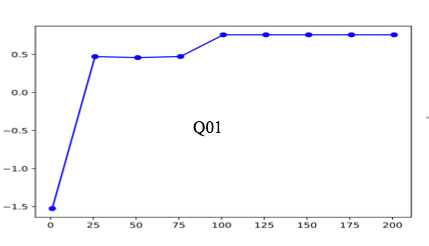
\includegraphics[height=1in,width=3in]{Figures/Q1.png}
	%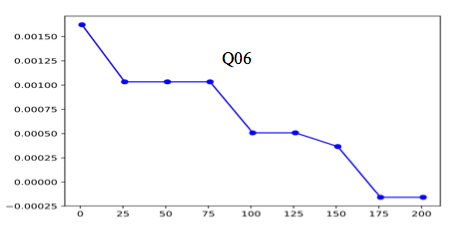
\includegraphics[height=1in,width=3in]{Figures/Q6.png}
	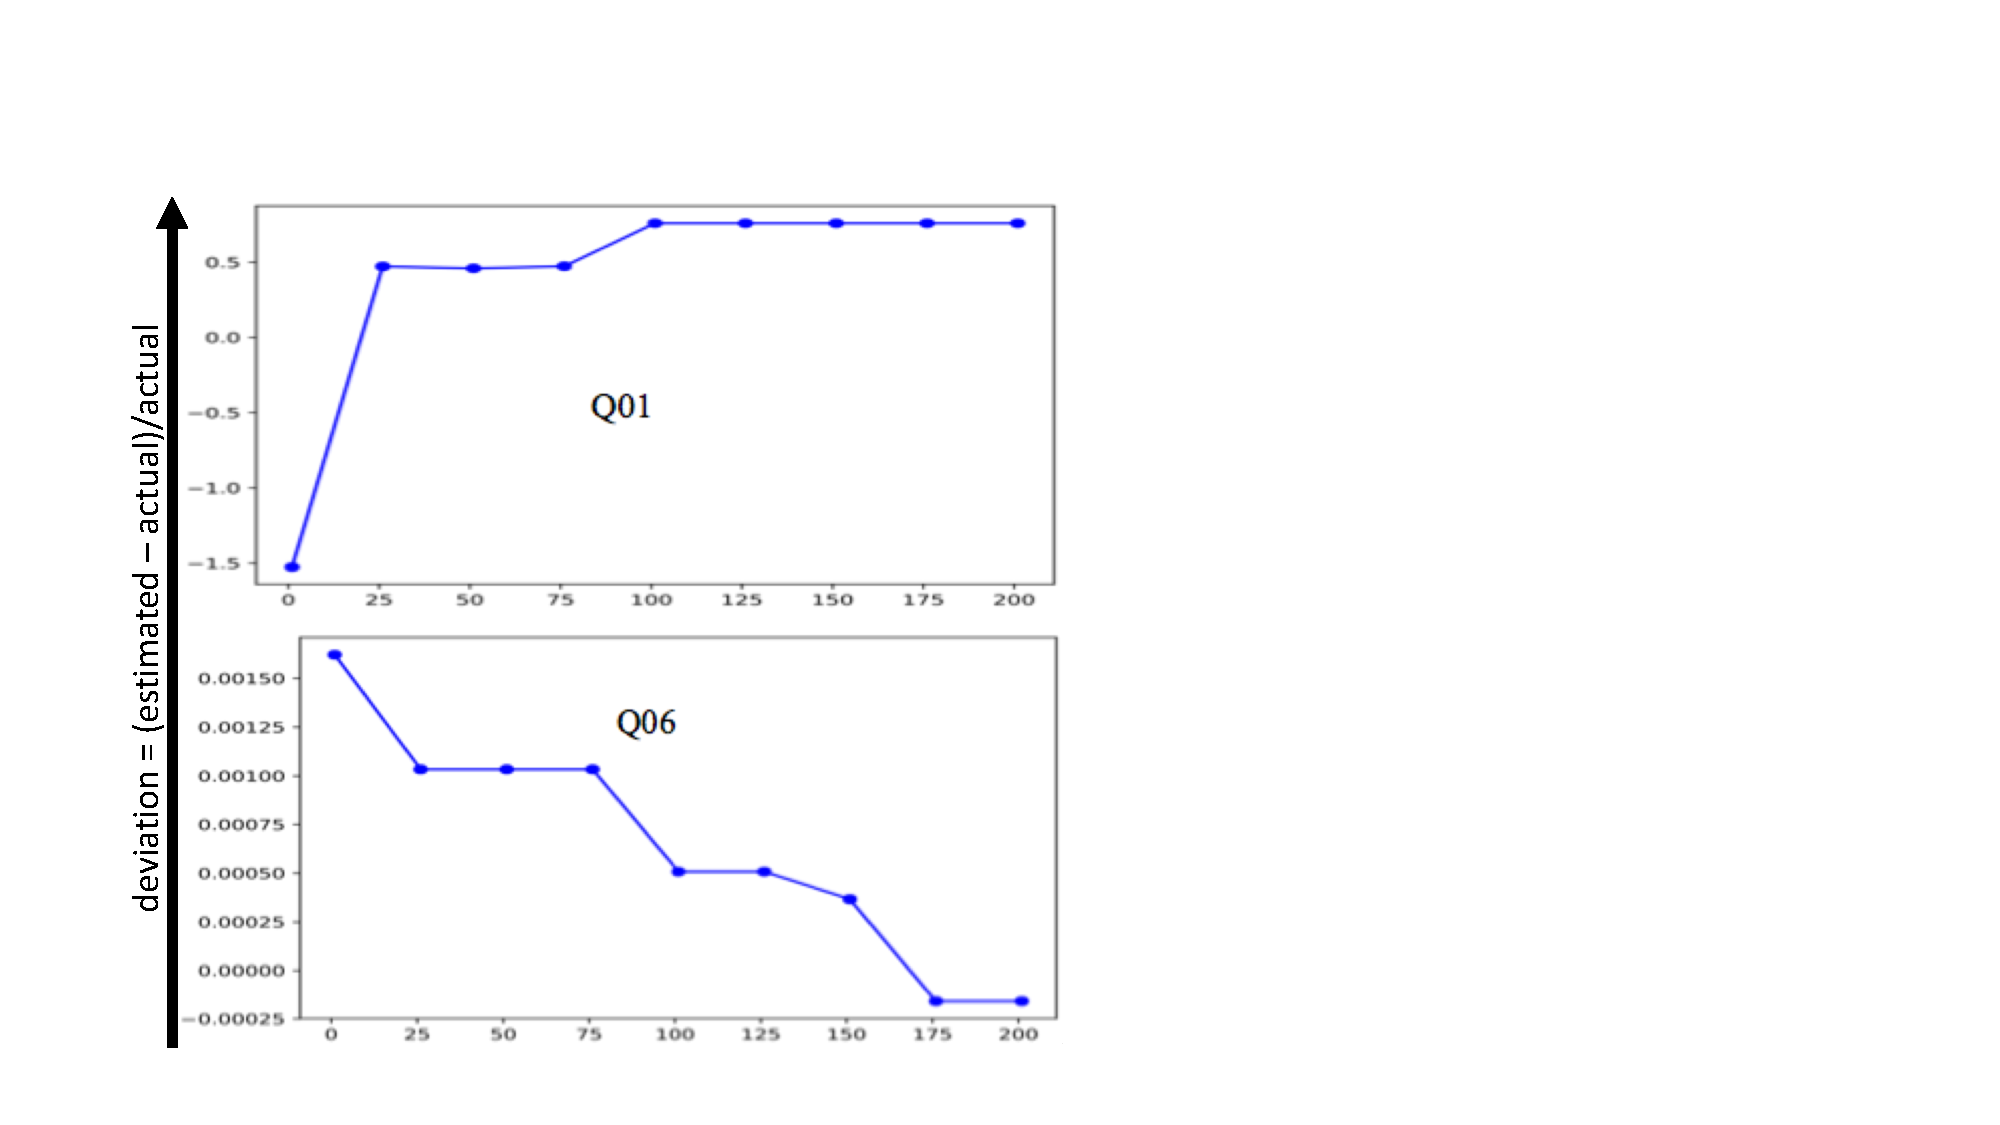
\includegraphics[width=0.95\columnwidth]{Figures/tpch-q1-q6.pdf}
	\caption{TPC-H queries Q1 and Q6 prediction deviations
		\label{fig:tpch-q1-q6}}
\end{figure}

To test {\sc malcolm} against TPC-H we created a query generator, which changes the parameters in the official benchmark queries.
A key factor is to understand how long it takes before {\sc malcolm}'s prediction converges to the actual memory footprint.
%Therefore, we used a large collection of morphed queries and split it into two portions: one is used by the simulator to train the micro-models, the other is used to assess their quality.
As a training set for each query, we randomised every selection point and range to produce 200 random versions of the query.
As a test set we used the original queries.

Initial experiments led to the results such as shown in Figure~\ref{fig:tpch-q1-q6}, where the x-axis shows the number of training queries used and y-axis shows the deviation of the estimation from the actual footprint.
Q1 is a simple large scan followed by an aggregation. The sole parameter is the value range.
The experiment shows a steep learning curve, which can be attributed to the uniform distribution.
However, it also results in a little overfitting.
Q6 is also mostly a simple scan and aggregate query, but here the number of tuples are less.
This experiment shows that {\sc malcolm} takes much longer to reach an almost perfect prediction of the memory footprint.

%In query 19 we observed a misprediction of 70\%.
%The reason is that the {\sc mal} algebra of this specific query consists of a lot of merge instructions, for which we output the sum of the two arguments, which in case of merging similar variables can lead to an almost 2$\times$ overestimation.
%This is the basic reason for the large error observed:
%\begin{verb}
%C_187 := algebra.thetaselect(X_178, "DELIVER IN PERSON", "==")
%X_191 := bat.mergecand(C_187, C_187)
%X_194 := bat.mergecand(X_191, C_187)
%\end{verb}
%[Move queries to appendix]
%\begin{verb}
%select l_returnflag, l_linestatus,
%       sum(l_quantity) as sum_qty,
%       sum(l_extendedprice) as sum_base_price,
%       sum(l_extendedprice * (1 - l_discount)) as sum_disc_price,
%       sum(l_extendedprice * (1 - l_discount) * (1 + l_tax)) as sum_charge,
%       avg(l_quantity) as avg_qty,
%       avg(l_extendedprice) as avg_price,
%       avg(l_discount) as avg_disc,
%       count(*) as count_order
%from lineitem
%where l_shipdate <= date '1998-12-01' - interval '90' day (3)
%group by l_returnflag, l_linestatus
%order by l_returnflag, l_linestatus;
%\end{verb}

%\begin{verb}
%select sum(l_extendedprice * l_discount) as revenue
%from lineitem
%where l_shipdate >= date '1994-01-01'
%  and l_shipdate < date '1994-01-01' + interval '1' year
%  and l_discount between .06 - 0.01 and .06 + 0.01
%  and l_quantity < 24;
%\end{verb}

\subsection{Air Traffic}
The air traffic benchmark is a real-world example of business intelligence application.
The data is represented by a single table, and it is highly skewed and sparse.
The queries are mostly simple select-group-aggregate, but given the table size still hard to process.
Figure~\ref{fig:airtraffic-q4-q15} and Figure~\ref{fig:airtraffic-q10-q19} show some of the results.
Again we can observe both some under- and over-estimations, which all improve over time.
Albeit they take more queries to stabilise.
%One immediate observation is that in this case it takes more queries to reach an optimal estimate.
% One with a deviation close to zero.
The graphs of Q04, Q15 and Q19 also illustrates how {\sc malcolm} not necessarily improves monotonicly.
This is most probably due to the actual query load.

\begin{figure}[t!]
	\centering
	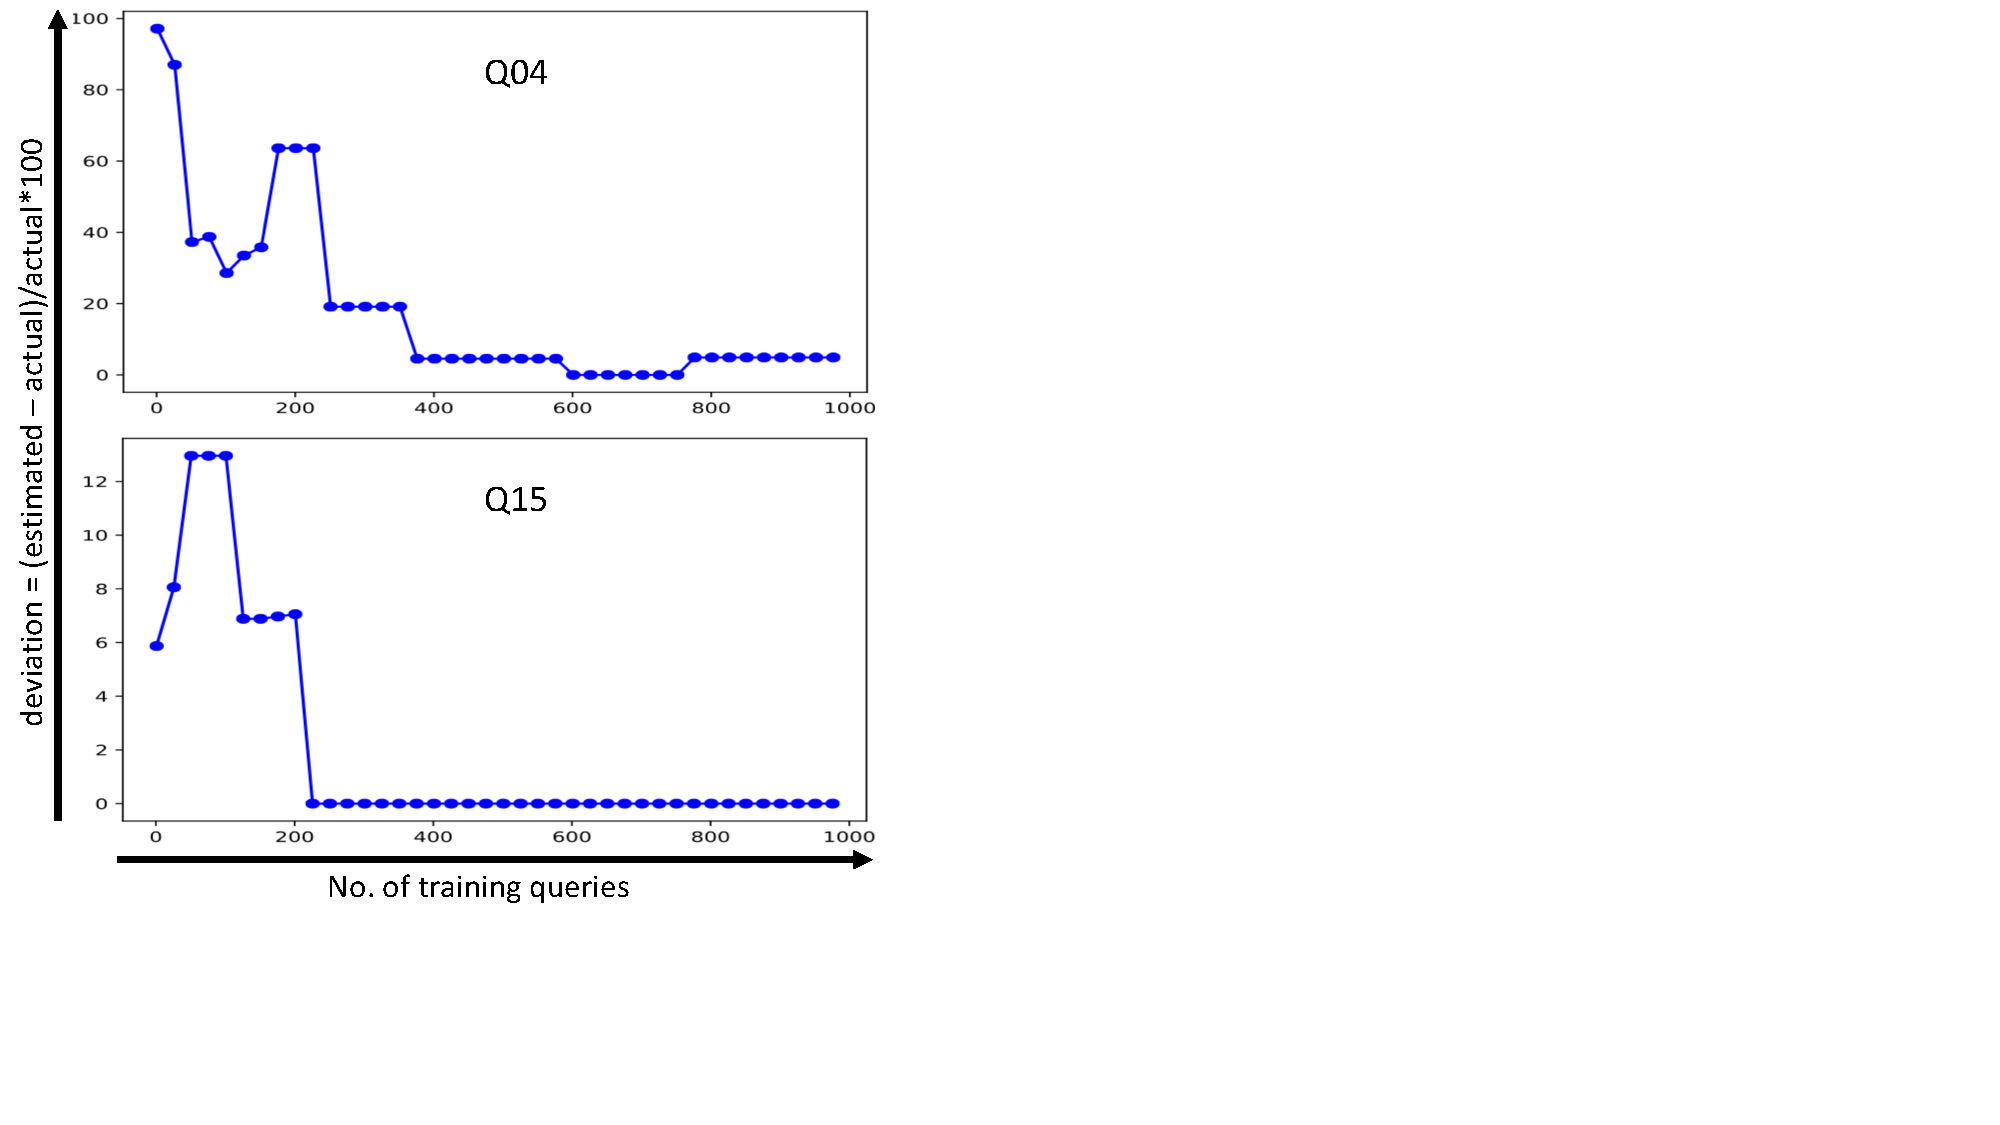
\includegraphics[height=2in,width=3in]{Figures/airtraffic-q4-q15.pdf}
	\caption{Air traffic queries 4 and 15
		\label{fig:airtraffic-q4-q15}}
\end{figure}

\begin{figure}[t!]
	\centering
	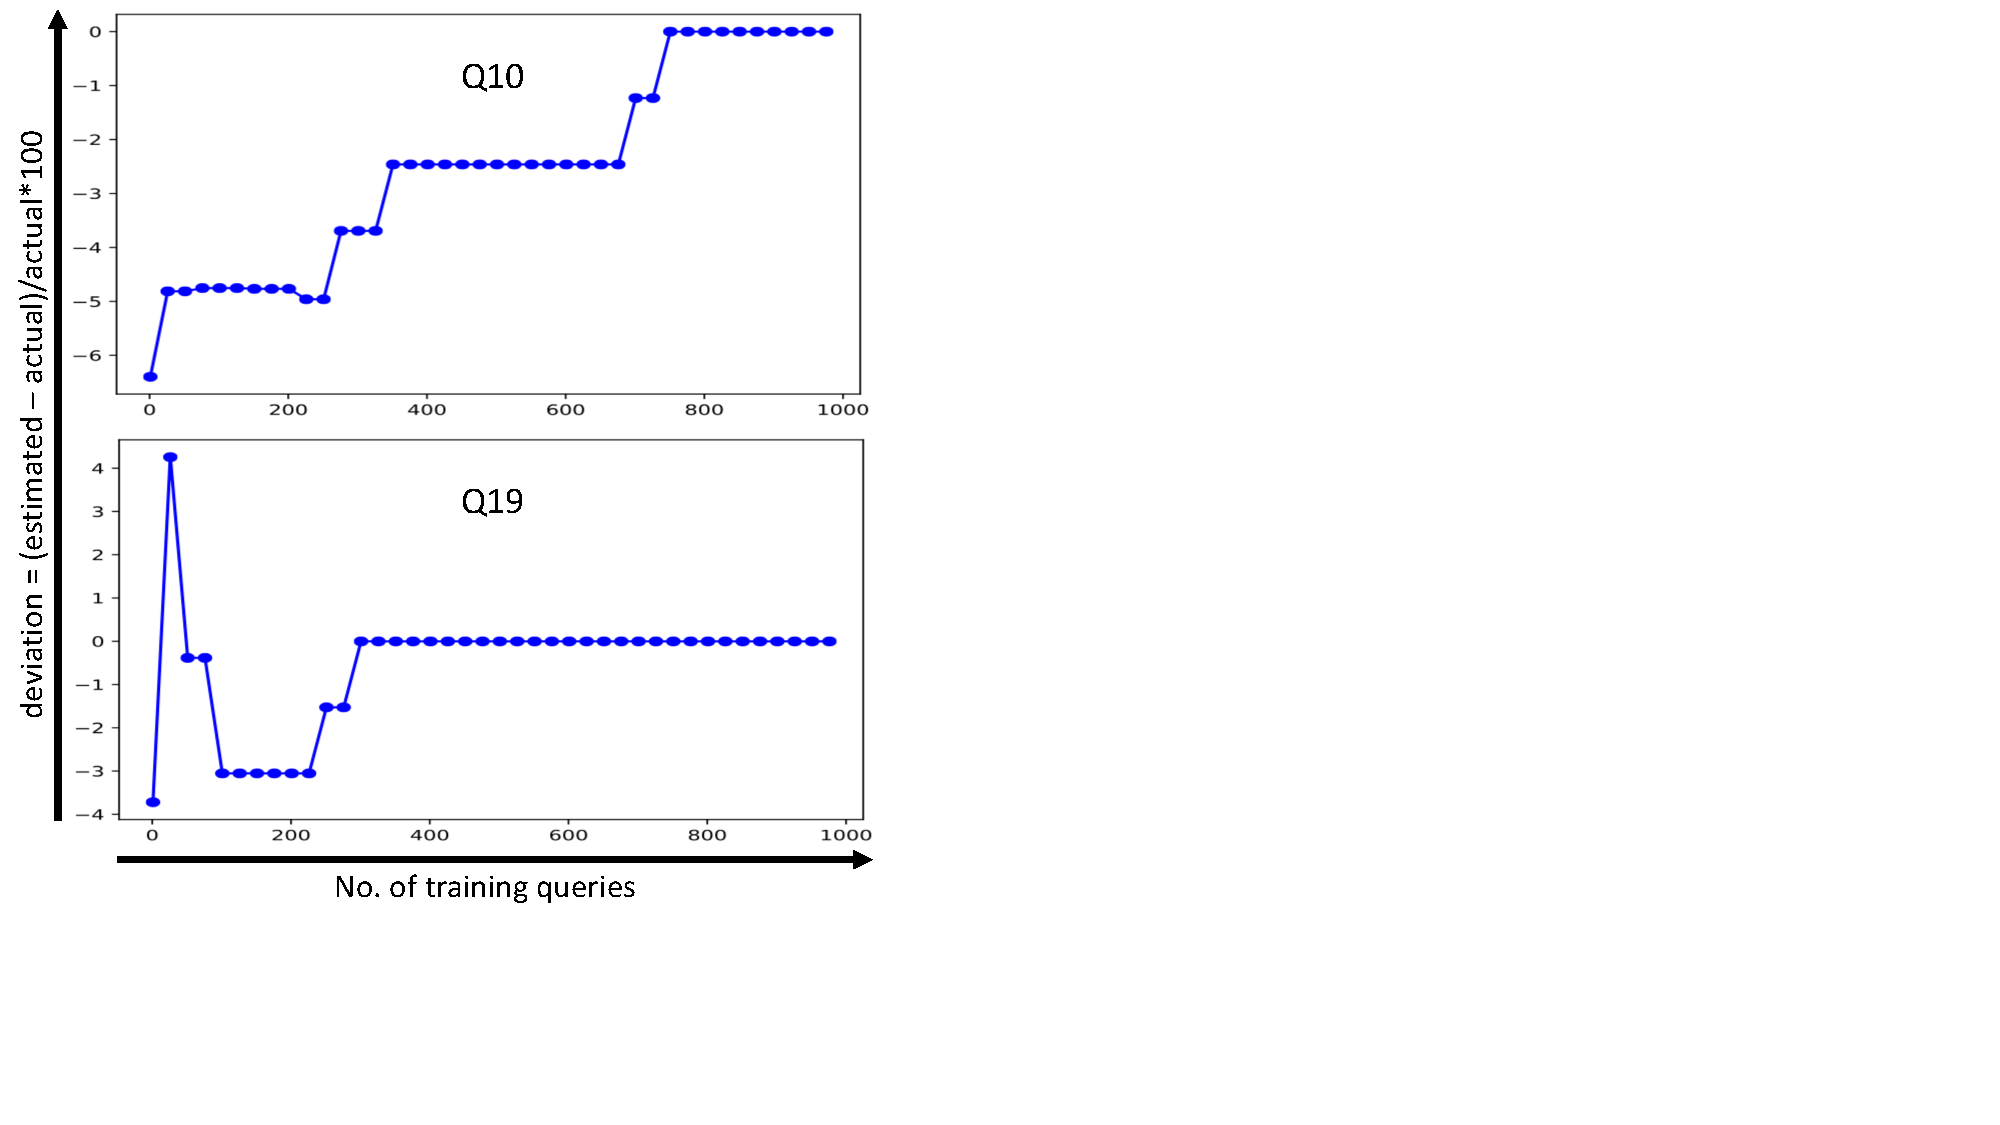
\includegraphics[height=2in,width=3in]{Figures/airtraffic-q10-q19.pdf}
	\caption{Air traffic queries 10 and 19
		\label{fig:airtraffic-q10-q19}}
\end{figure}

\section{Related work}
The approach taken in this project can best be compared with the long tradition in database query optimisers and database design wizards.
They all collect query traces from an actual production system and use them to derive e.g. an optimal set of search accelerators~\cite{DBLP:conf/vldb/ChaudhuriN07}.
This process seeks a balance between index creation and maintenance, but primarily deals with performance optimisation.
The memory footprint is of less concern.
Alternatively, it extends the work on gathering query traces to (semi-)automatically improve the cost model for query optimisation~\cite{DBLP:journals/ibmsj/MarklLR03}.
A better statistics improves both performance and resource use.
All these systems are focused on a relative small and fixed compute cluster or database appliance.

In a more recent project~\cite{DBLP:journals/pvldb/DingDWCN18} the authors gather sub-plans from the query trace log and use it as the building block for new queries.
They show that reuse of good plans, i.e. based on past behaviour, leads to both a faster optimisation step and overall better performance.
{\sc malcolm} does not address the optimiser itself, but assumes that a physical plan has already been produced.
It merely determines which virtual machine can handle the plan comfortably.

\section{Summary and Outlook\label{summary}} 
%In this paper we proposed a novel resource allocation technique for a database engine using resilient intermediates.
The {\sc malcolm} prototype is a crucial tool in the design of cloud-based database management solution.
The initial results are promising, a rather low number of queries are sufficient to get a good memory footprint estimate.

In the near future, we plan to extend {\sc malcolm} to also look at the memory footprint in relationship of the parallel execution.
%This should lead to a lower bound on the memory footprint at the cost of running slower.
Both memory footprint and degree of parallelism enables users to optimise their systems based on costs or response times.


% ensure same length columns on last page (might need two sub-sequent latex runs)
\balance

\section*{Acknowledgments}
This research has received funding from the European Union's Horizon 2020 research and innovation program under Grant Agreement no. 732366 (ACTiCLOUD).
\bibliography{IEEEabrv,refs}
\bibliographystyle{IEEEtran}

\end{document}
